\subsubsection{FOC-Treiber TMC4671}
\label{subsubsec:FOC-Treiber_TMC4671}

%Wie dem Grobkonzept in Kapitel \ref{subsec:Blockschaldbild} entnommen werden kann, wird für die Ansteuerung des BLDC-Motors eine Steuerlogik (Motor Control Unit) benötigt, welche die Gate-Ctrl-Signale erzeugt. Dabei handelt es sich um den TMC4671.
Der FOC-Treiber berechnet den Modulationsindex für die H-Brücke anhand des Drehmoments, der Geschwindigkeit oder der Position, welche der Mikrocontroller dem FOC-Treiber vorgibt. Als Feedback benötigt der FOC-Treiber den momentanen Strom durch zwei der drei Spulen und eine Information über die momentane Lage des Rotors. Die vom FOC-Treiber ausgehenden PWM-Leitungen gehen direkt auf den Gate-Treiber, welcher dann wiederum die MOSFETs ansteuert.
%Der dritte Strom wird mit dem Knotengesetz berechnet. Da der BLDC in Stern geschaltet ist gilt:
%\begin{equation}
%I_U + I_V + I_W = 0
%\end{equation}

Da das Gehäuse des IC's nur schwierig lötbar ist, wird ein Breakout-Board (BOB) verwendet.
Auf das Board und die darauf vorhandenen Schaltungen wird im Funktionsbeschrieb eingegangen.
\newpage
\paragraph{Schema}\label{par:Schaltungsaufbau_TMC4671}\mbox{}\\

Auf dem Breakout-Board sind diverse Anschlussmöglichkeiten vorhanden. Für den Cocktailmixer werden folgende Schnittstellen verwendet:

\begin{itemize}
\item SPI Input
\item Phasenströme Input
\item Encoder Input
\item Motorspannung Input
\item Steuersignale Output
\end{itemize}

In der schon gezeigten Abbildung \ref{fig:Blockdiagramm_Motorengruppe} ist zu erkennen, welche Funktionen im Treiber vorhanden sind und wie diese zusammenhängen. Im wesentlichen kann daraus entnommen werden, dass der TMC4671 aus einer FOC-Logik\footnote{FOC= \textbf{F}ield \textbf{O}riented \textbf{C}ontrol}, einer Servo-Logik, einem SPI-Interface und diversen Engines (PWM, ADC, Encoder) besteht. Im Anhang Kapitel \ref{Appendix:Schaltung_TMC4671} wird eine Standard-Anwendungsschaltung gezeigt, worin erkennbar ist, dass der Treiber sehr universell aufgebaut ist und für mehrere Motorentypen verwendet werden können. Die für den PartyMixer essentiellen Ein- und Ausgänge wurden schon genannt.

In Abbildung \ref{fig:Schema_FOC_Treiber} ist erkennbar, welche Pins für den PartyMixer verwendet werden. Es handelt sich dabei um die schon aufgelisteten Komponenten, nämlich Kommunikationsleitung zwischen Treiber und Mikrocontroller (SPI), Phasenströme (ADC), Encoder Input (ENC), Motorspannung (48V) und das Gate-Ctrl-Signal (PWM).

\begin{figure}[H]
	\centering
	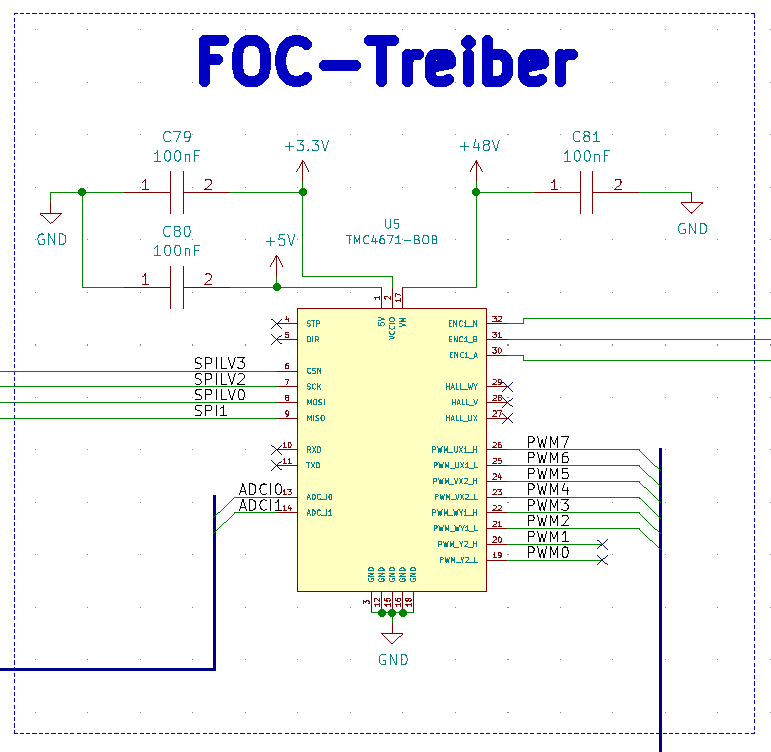
\includegraphics[width=0.7\textwidth]{graphics/Schema_FOC_Treiber}
	\caption{Schema FOC-Treiber.}
	\label{fig:Schema_FOC_Treiber}
\end{figure} 

\paragraph{Funktionsbeschrieb der Schaltung}\mbox{}\\

Im Folgenden werden kurz die Teilsysteme auf dem TMC4671-BOB beschrieben, welche für den Cocktailmixer gebraucht werden. Dazu wird auf das Layout vom Trinamic TMC4671-BOB zurückgegriffen. Sämtliche Teilschemas sind im Anhang Kapitel \ref{Appendix:BOB} aufgezeigt. \cite{trinamicmotion_control_gmbh__co_kg_tmc4671-bob_2020}

%\subparagraph{Kommunikation Input (SPI)}

Der SPI-Kommunikationseingang ist nicht speziell geschützt. Hier ist für das eigene Layout darauf zu achten, dass die angelegte Spannung nicht über 3.3V steigt. Dies wird mit einem Level-Shifter zwischen Mikrocontroller und TMC4671 gewährleistet.

%\subparagraph{Ströme Input (ADC)}

Der Eingang zur Strommessung ist mit einem Tiefpass geschützt. Dieser hat die Zeitkonstante:

\begin{equation}
\tau = R308 \cdot C300 = 100\Omega \cdot 100pF = 10ns
\end{equation}

%\subparagraph{Encoder Input (ENC)}

Um den Eingang der Encoder-Pins zu schützen, wird ein Schmitt-Trigger mit eingebautem Level-Shifter verwendet. Zudem wird mit dem Widerstandsnetzwerk ein entprellen der Encoder-Signale erreicht. Wird der Input auf 0V gezogen, so entlädt sich der Kondensator über die Widerstände R200-R202 mit der Zeitkonstante:

\begin{equation}
\tau = R200 \cdot C204 = 1k\Omega \cdot 100pF = 100ns
\end{equation}

Sobald der Eingang vom Encoder nicht mehr auf 0V gezogen wird, so lädt sich der Kondensator über die Widerstände R200-R202 sowie R206,R208,R210. Somit ergibt sich eine längere Zeitkonstante:

\begin{equation}
\tau = (R200 + R210) \cdot C204 = (1k\Omega + 4.7k\Omega) \cdot 100pF = 570ns
\end{equation}

Jetzt geht es bedeutend länger, bis der Kondensator wieder geladen wird. Sobald die Spannung wieder einen bestimmten Wert erreicht, wird der Schmitt-Trigger aktiv und springt auf Versorgungsspannung (3.3V). Im Anhang Abbildung \ref{fig:Schmitt_Trigger_Debounce} ist die Funktion verdeutlicht.

%\subparagraph{Motorspannung Input (48V)}

Die Motorspannung ist wichtig, um den Kommuntierungsvorgang zu berechnen. Wichtiger als die Zeitkonstante ist hier ein Spannungsteiler, welcher die Motorspannung auf unter 3.3V bringt. Dazu wird folgende Formel angewendet:
\todo{Filter vorhanden, siehe datenblatt}

\begin{equation}
U_{TMC} = U_M \cdot \frac{R310}{R310 + R311} = 48V \cdot \frac{1k\Omega}{1k\Omega + 100k\Omega} = 0.7V
\end{equation}

%\subparagraph{Gate-Ctrl-Signale Output (PWM)}

Die Ausgangssignale für den Gate-Treiber gehen direkt auf die Header-Pins des TMC4671-BOB.

%\subsubsection{Encoder-Input}\label{subsubsec:Encoder_Input}
%
%Vor einem Analogeingang wird das Signal in der Regel mit einem Tiefpass gefiltert, um stochastische Abweichungen zu verhindern. Dafür werden die Widerstände \textbf{R700-R702} und die Kondensatoren \textbf{C700-C702} verwendet. Die Beschaltung und Dimensionierung wurde aus dem Datenblatt des TMC4671-EVAL-Board entnommen. Die Zeitkonstante des Filters beträgt gemäss Formel \ref{equ:Berechnung_Encoder_LP} 10ns. Das Schaltungsprinzip ist in Abbildung \ref{fig:Schema_Encoder_LP} dargestellt. 
%\begin{equation}
%\tau = R \cdot C = 100\Omega \cdot 100\cdot10^{-12}F = 10 \cdot 10^{-9}s = 10ns
%\label{equ:Berechnung_Encoder_LP}
%\end{equation}
%
%Der Motor hat eine Drehzahl von max. 1500rpm, dies entspricht einer maximalen Periodendauer von $\mathrm{666.\overline{6} \mu}$s. Das Eingangssignal wird deshalb nicht herausgefiltert.
%
%Die Komponenten \textbf{D700-D702} sind Bauteile, welche zwei Shottky-Dioden verbaut haben und sind dazu da, eventuell auftretende Über-/ und Unterspannungen zu verhindern. Abbildung \ref{fig:Schema_Encoder_2_LP} zeigt die Anordnung der internen Dioden an Stelle des
%verwendeten Bauteils. Jede Diode hat eine Durchlassspannung von 0.3V. Liegt in Abbildung \ref{fig:Schema_Encoder_2_LP} beim Eingangssignal eine Spannung von über 5.3V an, wird die Diode an 5V leitend und verhindert ein weiteres Ansteigen der Eingangsspannung. Das Selbe bei Unterspannung, sobald eine Spannung von -0.3V anliegt, wird die Diode an 0V leitend, und verhindert ein weiteres Absinken der Spannung.

%\begin{figure}[h!]
%	\centering	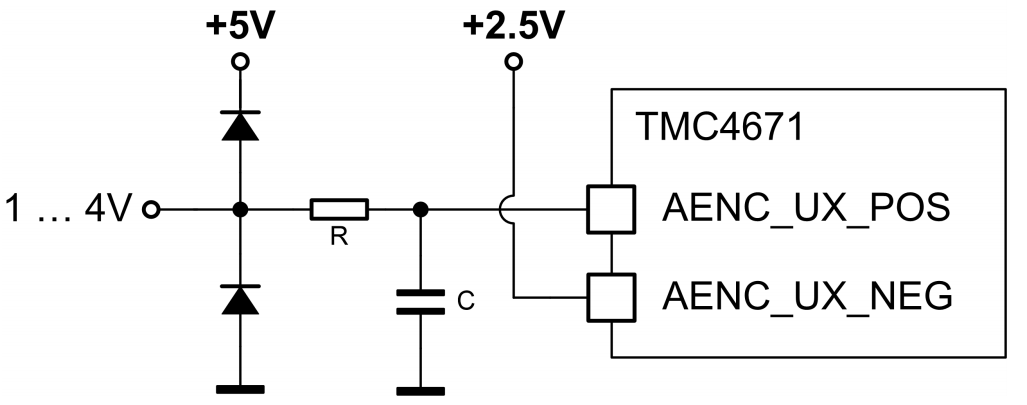
\includegraphics[width=0.5\textwidth]{graphics/Schema_Encoder_2_LP.png}
%	\caption{Teilschema aus Datenblatt TMC4671. Hier mit Shottky-Dioden anstelle IC.}
%	\label{fig:Schema_Encoder_2_LP}
%\end{figure}

%Die Widerstände \textbf{R703-R708} Stellen Spannungsteiler dar, welche gemäss Datenblatt eine benötigte Spannung von 2.5V bereitstellen.
%
%Der Kondensator \textbf{C703} ist ein Stützkondensator und dient der Speisung eines Ecoders. Die Versorgungsspannung wird jedoch nicht für den Resolver benötigt.
%
%Der Header \textbf{J6} ermöglicht, den Resolver an das PCB anzuschliessen.
%
%Abbildung \ref{fig:Schema_Encoder_LP} zeigt das Gesamte Schema mit den Komponenten, welche ein korrektes Einlesen des Resolvers ermöglichen.

%\begin{figure}[h!]
%	\centering	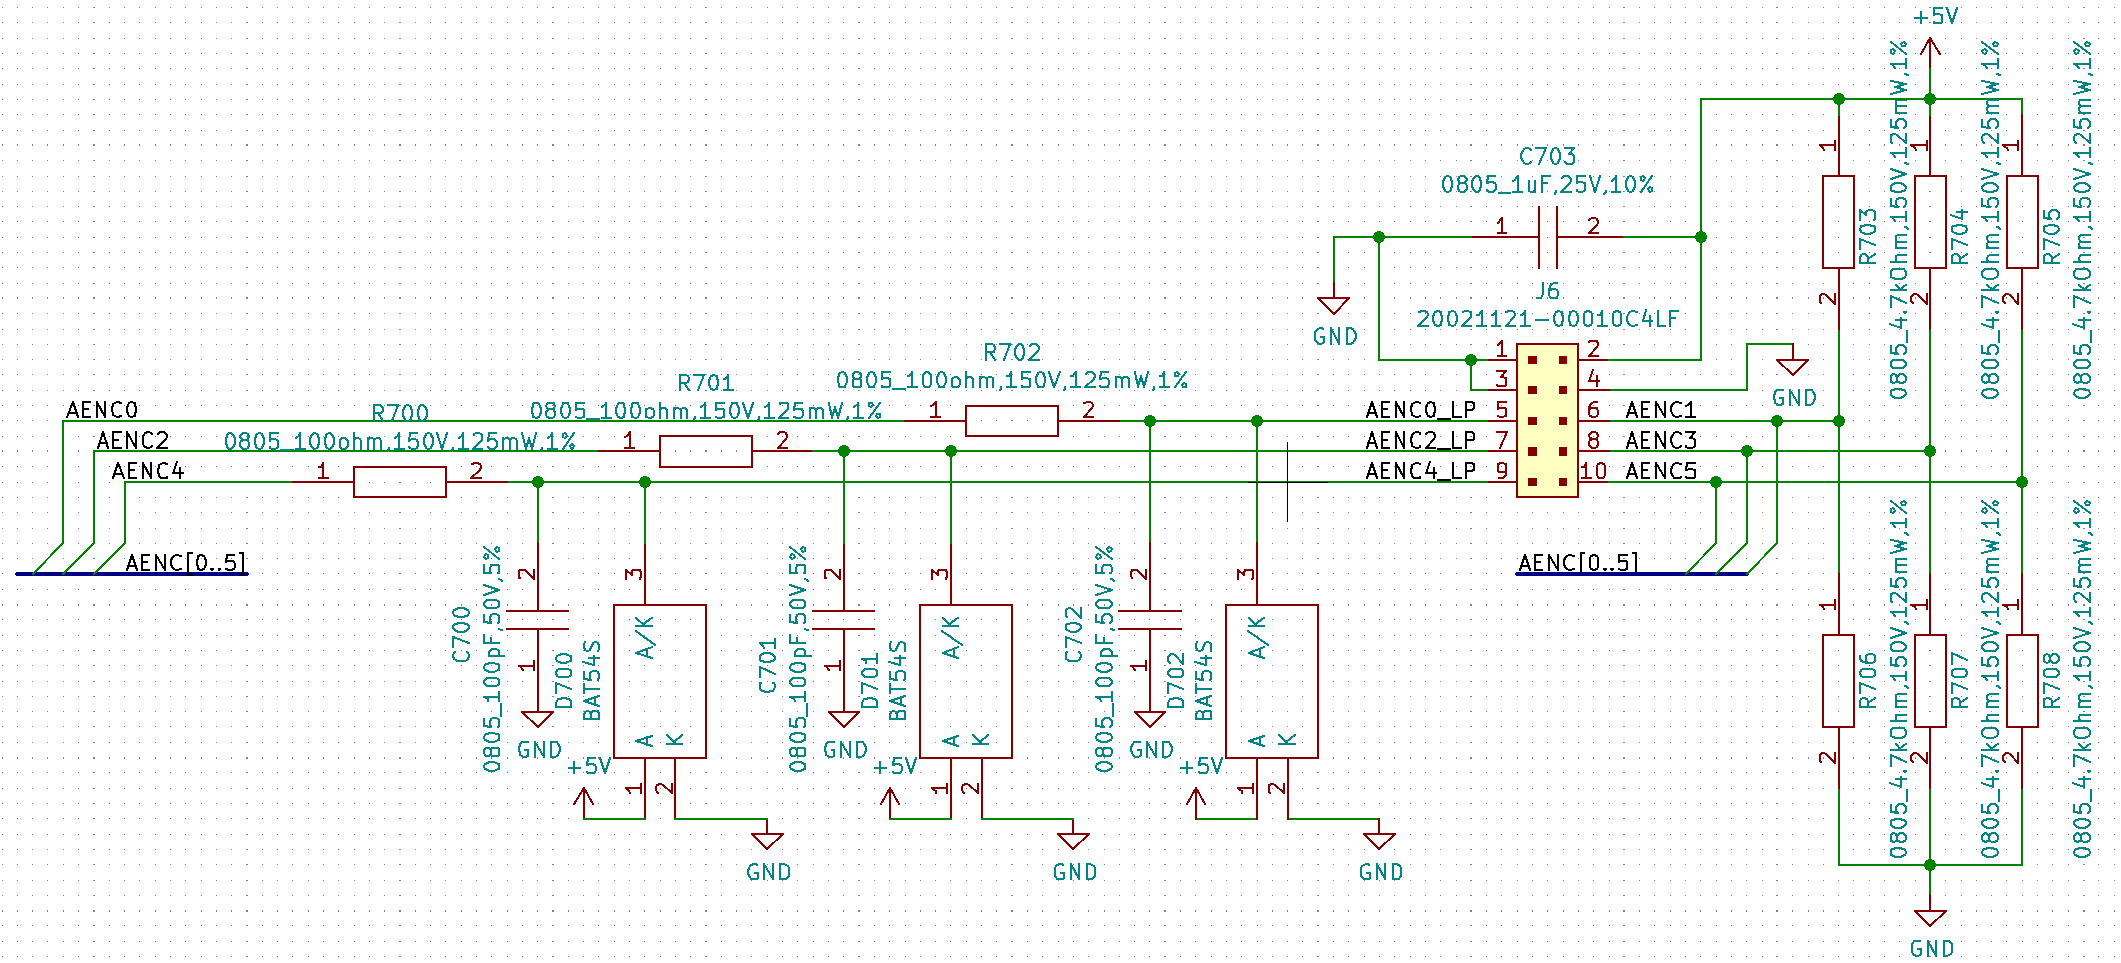
\includegraphics[width=\textwidth]{graphics/Schema_Encoder_LP.png}
%	\caption{Teilschema TMC4671. Hier Input Encoder.}
%	\label{fig:Schema_Encoder_LP}
%\end{figure}

%\subsubsection{Analog-Inputs}\label{subsubsec:Analog_Inputs}
%
%Auch hier wird das Eingangssignal mit einem Tiefpass gefiltert. Dafür werden die Widerstände R711 und R713 sowie die Kondensatoren C707 und C709 verwendet. Die Beschaltung und Dimensionierung wurde aus dem Datenblatt des TMC4671-EVAL-Board entnommen. Die Zeitkonstante des Filters beträgt gemäss Formel \ref{equ:Berechnung_Analog_LP} 400ns. Das Schaltungsprinzip ist in Abbildung \ref{fig:Schema_Analog_LP} dargestellt. \cite[PDF S.25]{trinamic_drawings_2018}
%\begin{equation}
%\tau = R \cdot C = 4\cdot 10^{3}\Omega \cdot 100\cdot10^{-12}F = 10 \cdot 10^{-9}s = 400ns
%\label{equ:Berechnung_Analog_LP}
%\end{equation}
%
%Weiter befindet sich ein zweiter Widerstand in jeder Schaltung
%\todo{Funktion zweiter Widerstand herausfinden.}
%
%Das letzte Bauteil, welches noch beschrieben werden muss, sind die Dioden D703 und D704. Diese stellen jeweils wieder einen Über- bzw. Unterspannungsschutz dar, um den Messeingang des TMC4671 zu schützen. Das Bauteil ist das selbe wie oben im Encoder-Teil, weshalb hier auf eine tiefere Beschreibung verzichtet wird.
%
%\begin{figure}[h!]
%	\centering	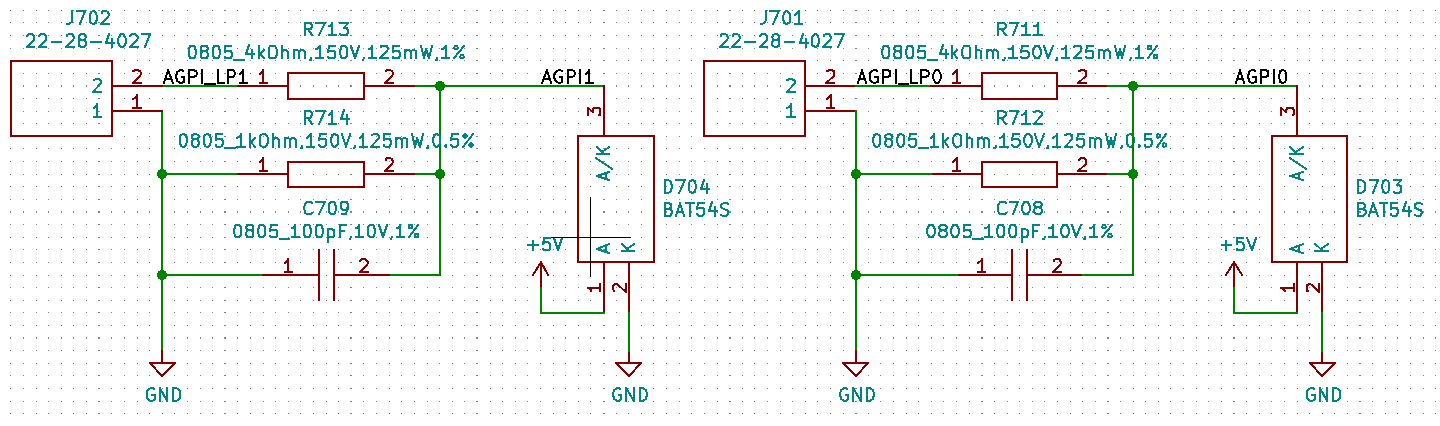
\includegraphics[width=0.8\textwidth]{graphics/Schema_Analog_Inputs_LP.png}
%	\caption{Teilschema TMC4671. Hier Inputs Analog.}
%	\label{fig:Schema_Analog_LP}
%\end{figure}
%
%
%\subsubsection{Motorspannung-Input}\label{subsubsec:Motorspannung_Input}
%
%\cite[PDF S.25]{trinamic_drawings_2018}
%\begin{figure}[h!]
%	\centering	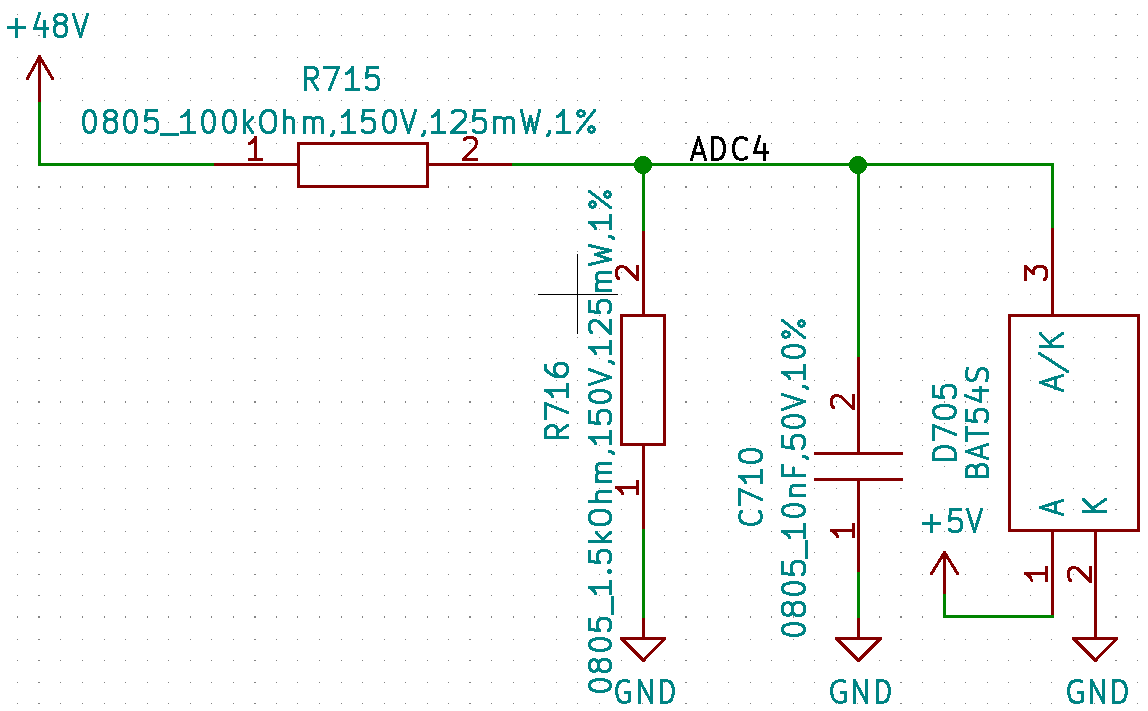
\includegraphics[width=0.45\textwidth]{graphics/Schema_VM_Input_LP.png}
%	\caption{Teilschema TMC4671. Hier Input Motorspannung.}
%	\label{fig:Schema_Encoder_LP}
%\end{figure}